\documentclass[]{article}
\usepackage[english]{babel}
\usepackage{graphicx}
\usepackage{subfig}
\usepackage{tabularx}
\usepackage{listings}
\usepackage[]{hyperref}

\addto\extrasenglish{%
  \def\subsectionname{section}%
  \def\subsectionautorefname{section}%
  \def\subsubsectionname{section}%
  \def\subsubsectionautorefname{section}%
}

\newcommand*{\fullref}[1]{\hyperref[{#1}]{\autoref*{#1} \nameref*{#1}}}

\lstdefinelanguage{JavaScript}{
  keywords={break, case, catch, continue, debugger, default, delete, do, else, finally, for, function, if, in, instanceof, new, return, switch, this, throw, try, typeof, var, void, while, with},
  morecomment=[l]{//},
  morecomment=[s]{/*}{*/},
  morestring=[b]',
  morestring=[b]",
  sensitive=true
}

\hypersetup{
  colorlinks=true,  % links sind farbig und haben keine umrandung
  linkcolor=[rgb]{0,0.2,0.4}, % dunkelblaue farbe für dokumenten interne links
  urlcolor=blue % url links sind blau
}

%opening
\title{Voxie - User Manual}
\author{}

\begin{document}

\maketitle

\section{Table Of Contents}
\tableofcontents
\newpage

\section{Introduction}
This document explains the features of Voxie and how they can be used.

\section{Overview}
Voxie is a voxel volume viewer designed to process and visualize 3D Images created from tomography.
\\
It's main focus is set on extracting 2 dimensional slice images from slices with arbitrary rotation and position within a 3D Image.

\section{User Interface}
% TODO BY FELIX

The following chapter will describe the graphical user interface of Voxie.

\subsection{Windows}

Voxie is an application built around one main window. It contains all main
features like showing visualizers and the runtime configuration in the
side panel.

\subsubsection{Main Window}

\begin{figure}[h]
  \centering
  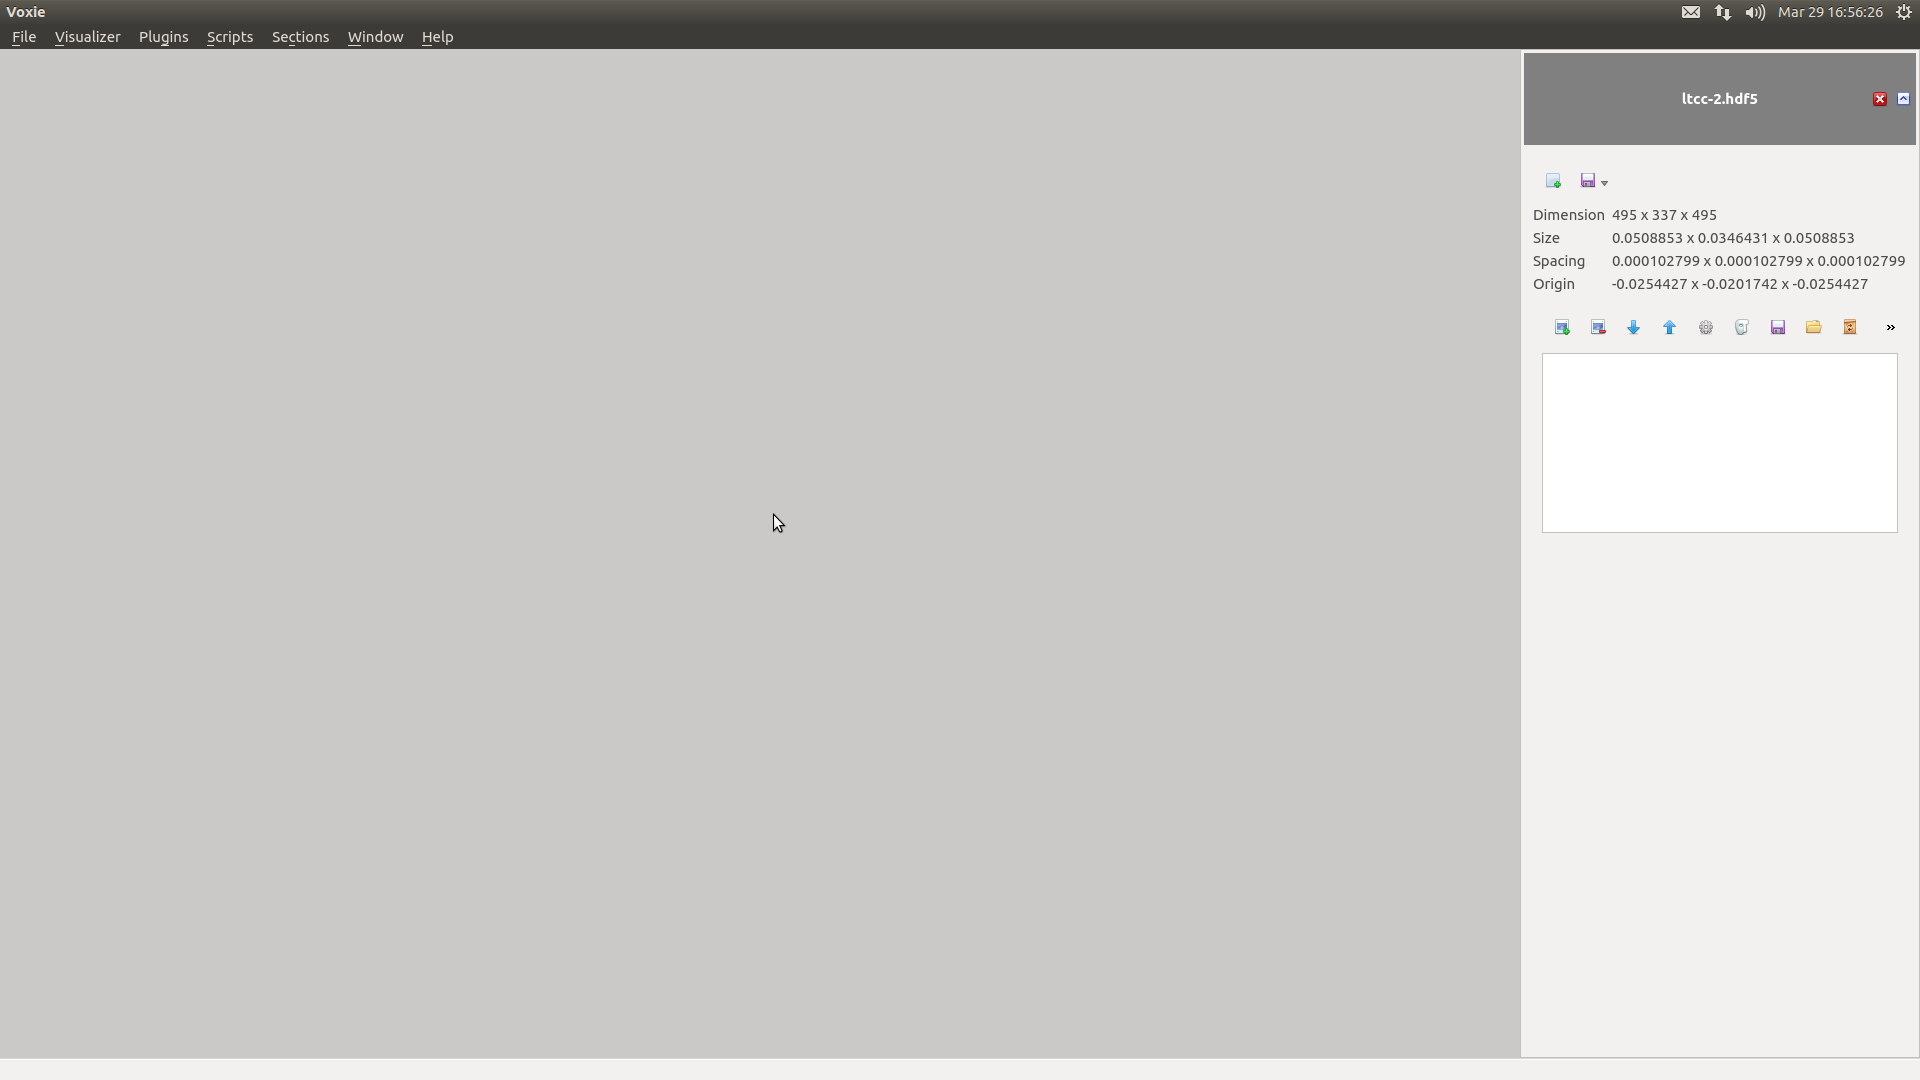
\includegraphics[width=1.0\textwidth]{img/mainwindow.png}
  \caption{Main Window}
\end{figure}

The main window opens when Voxie gets started. It contains the main menu,
the side panel and shows all open visualizers in the center.

The side panel is described further in \ref{sections}.

The main menu is described futher in \ref{menus}.

\subsubsection{Preferences Window}
\label{preferences-window}

The preferences window allows the user to modify and customize Voxie for
his needs.

It allows setting up custom script types for external script files, select the
used OpenCL devices and options provided by plugins.

\begin{figure}[h]
  \centering
  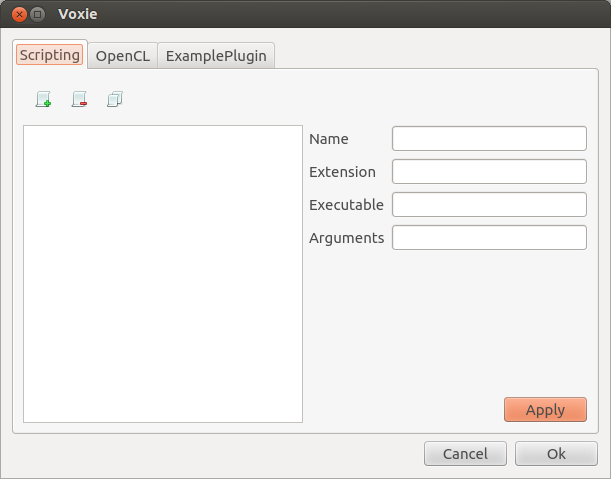
\includegraphics[width=0.6\textwidth]{img/preferences-script.png}
  \caption{Preferences Window}
\end{figure}

\subsubsection{Scripting Window}
\label{scripting-window}

The scripting window provides a small JavaScript console for live scripting.
A line of code can be entered in the bottom text box and with a click on \emph{Run!}
or a on the return key, the script will be executed.
It is possible to navigate through previously executed commands by pressing the up or
down arrow key.

It also shows a live debug log from running scripts.

\begin{figure}[h]
  \centering
  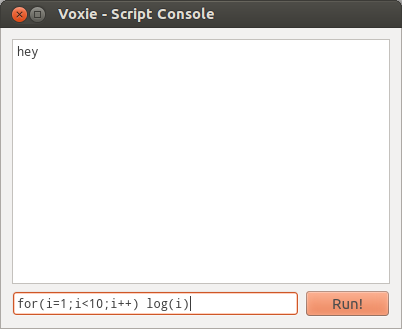
\includegraphics[width=0.5\textwidth]{img/script-console.png}
  \caption{Scripting Window}
\end{figure}


\subsubsection{Visualizer Windows}

Visualizer windows are a special kind of window.
Each visualizer can be separated from the main window
as a standalone window.

Those visualizer windows behave like the integrated windows
except they can be positioned anywhere on the work space
(including other monitors).

Separating a window can be achieved by clicking the "Detach" button
on top of each visualizer.
To re--attach a window the "Attach" button can be clicked on, which is located in the top left corner on any surface.

\subsection{Menus}
\label{menus}

\subsubsection{File}

The file menu contains the main control of Voxie as well as options to load
files.

To load a file, there are two options:
\begin{itemize}
  \item{Loading a file}
  \item{Using an importer}
\end{itemize}
Loading a file always shows a file dialog (Fig. \ref{file-dialog}) which allows selection of
all plugin supported file types. Most options show an additional dialog after
confirming the dialog to make further settings on opening the file.

Example:\newline
The HDF5 importer shows a dialog for selection of the dataset as can bee
seen in Fig. \ref{hdf5-dialog}.

Using importers allows a more flexible way of loading data sets.
Importers are not bound to any predefined procedures, they can show any
kind of UI and allow advanced loading of data sets, e.g. like loading a data
set from multiple files, reading a data set from an external device or 
even just create a data set on the fly.

The file menu also contains an option to quit Voxie and another to set up
preferences for Voxie itself as well as for plugins that support options.

The ``New...'' option will close any open datasets to reset the workspace.

\medskip

Furthermore, the file menu contains the ability to save and load Voxie projects.

\begin{itemize}
  \item{Save Voxie Project}
  \item{Load Voxie Project}
\end{itemize}

Voxie projects are saved as Javascript files. These script files can be loaded at a 
later time to restore the saved session, with all its datasets, visualizers, and settings.
Note that the datasets themselves do not get saved with a project due to their size, 
these files need to be present on the hard drive in order to load a project.


\begin{figure}[!htbp]
  \centering
  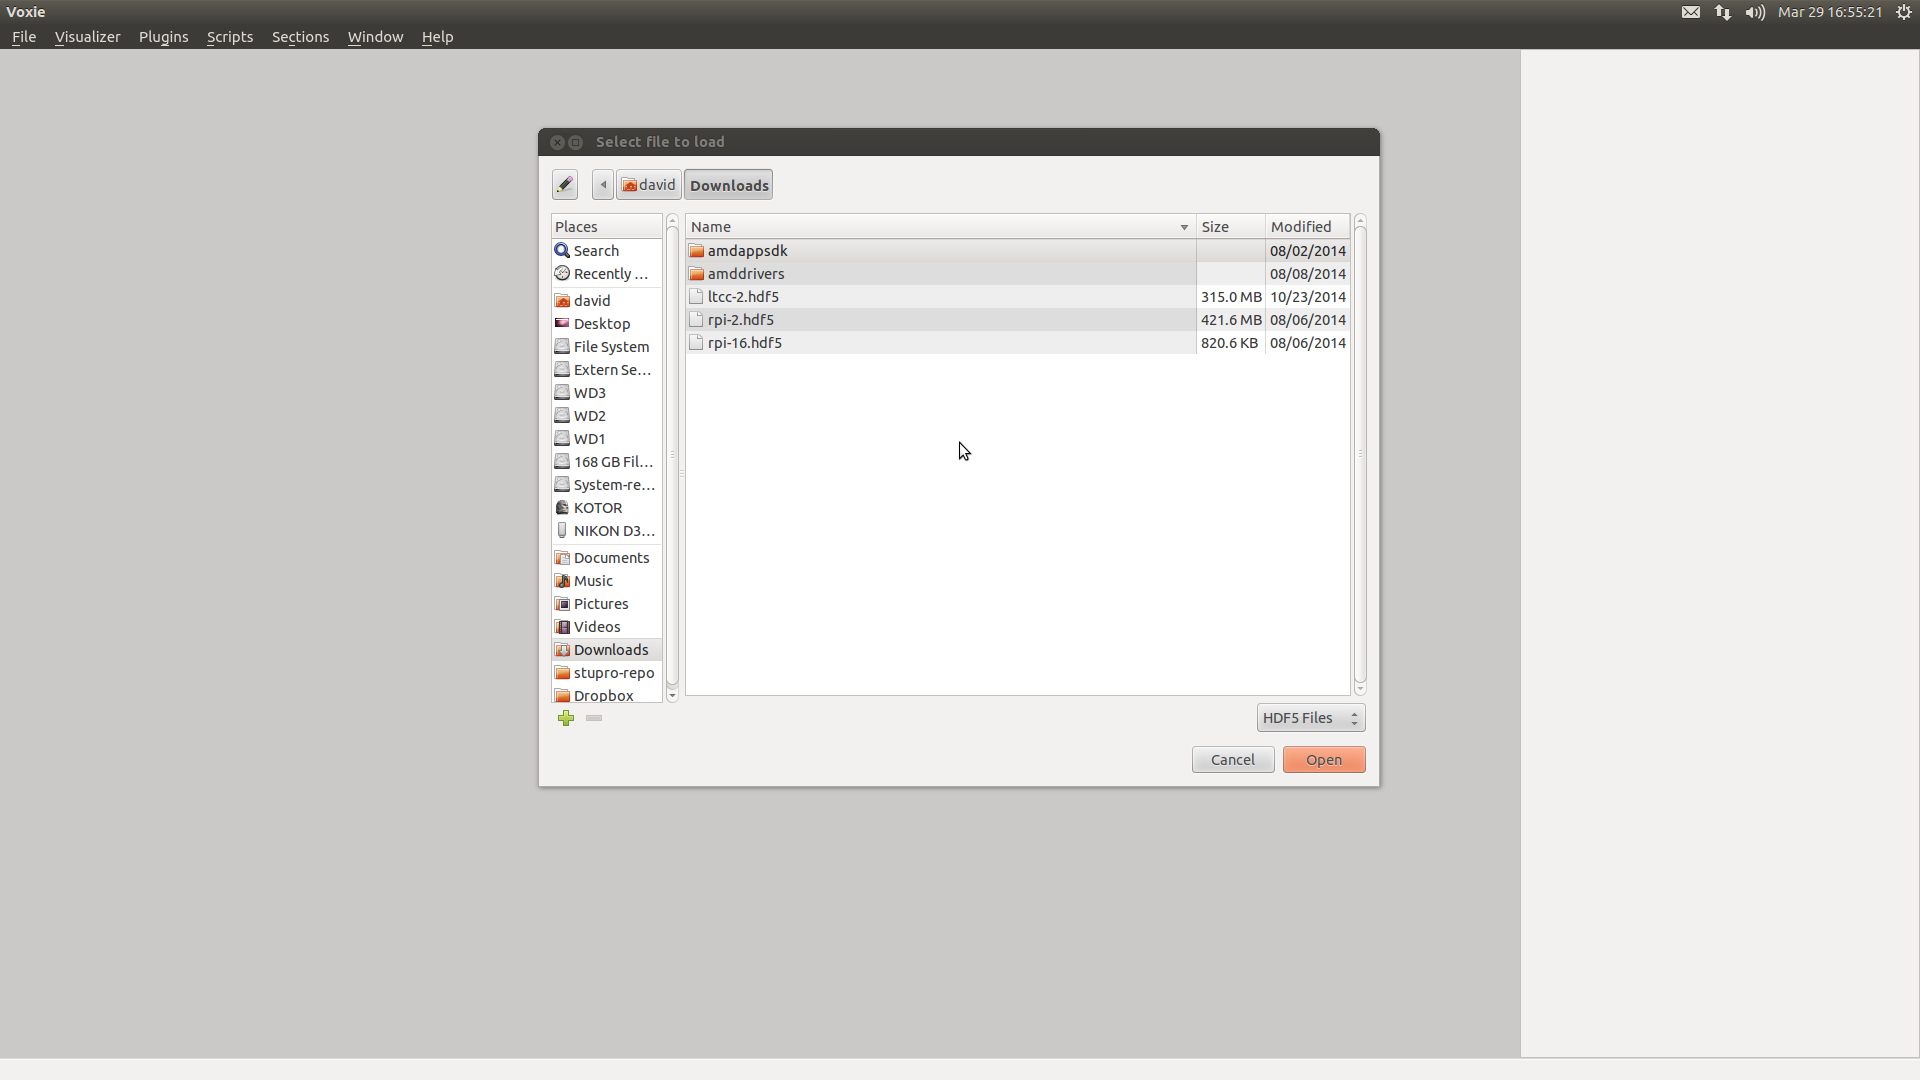
\includegraphics[width=1.0\textwidth]{img/file-dialog.png}
  \caption{File Dialog}
  \label{file-dialog}
\end{figure}

\begin{figure}[!htbp]
  \centering
  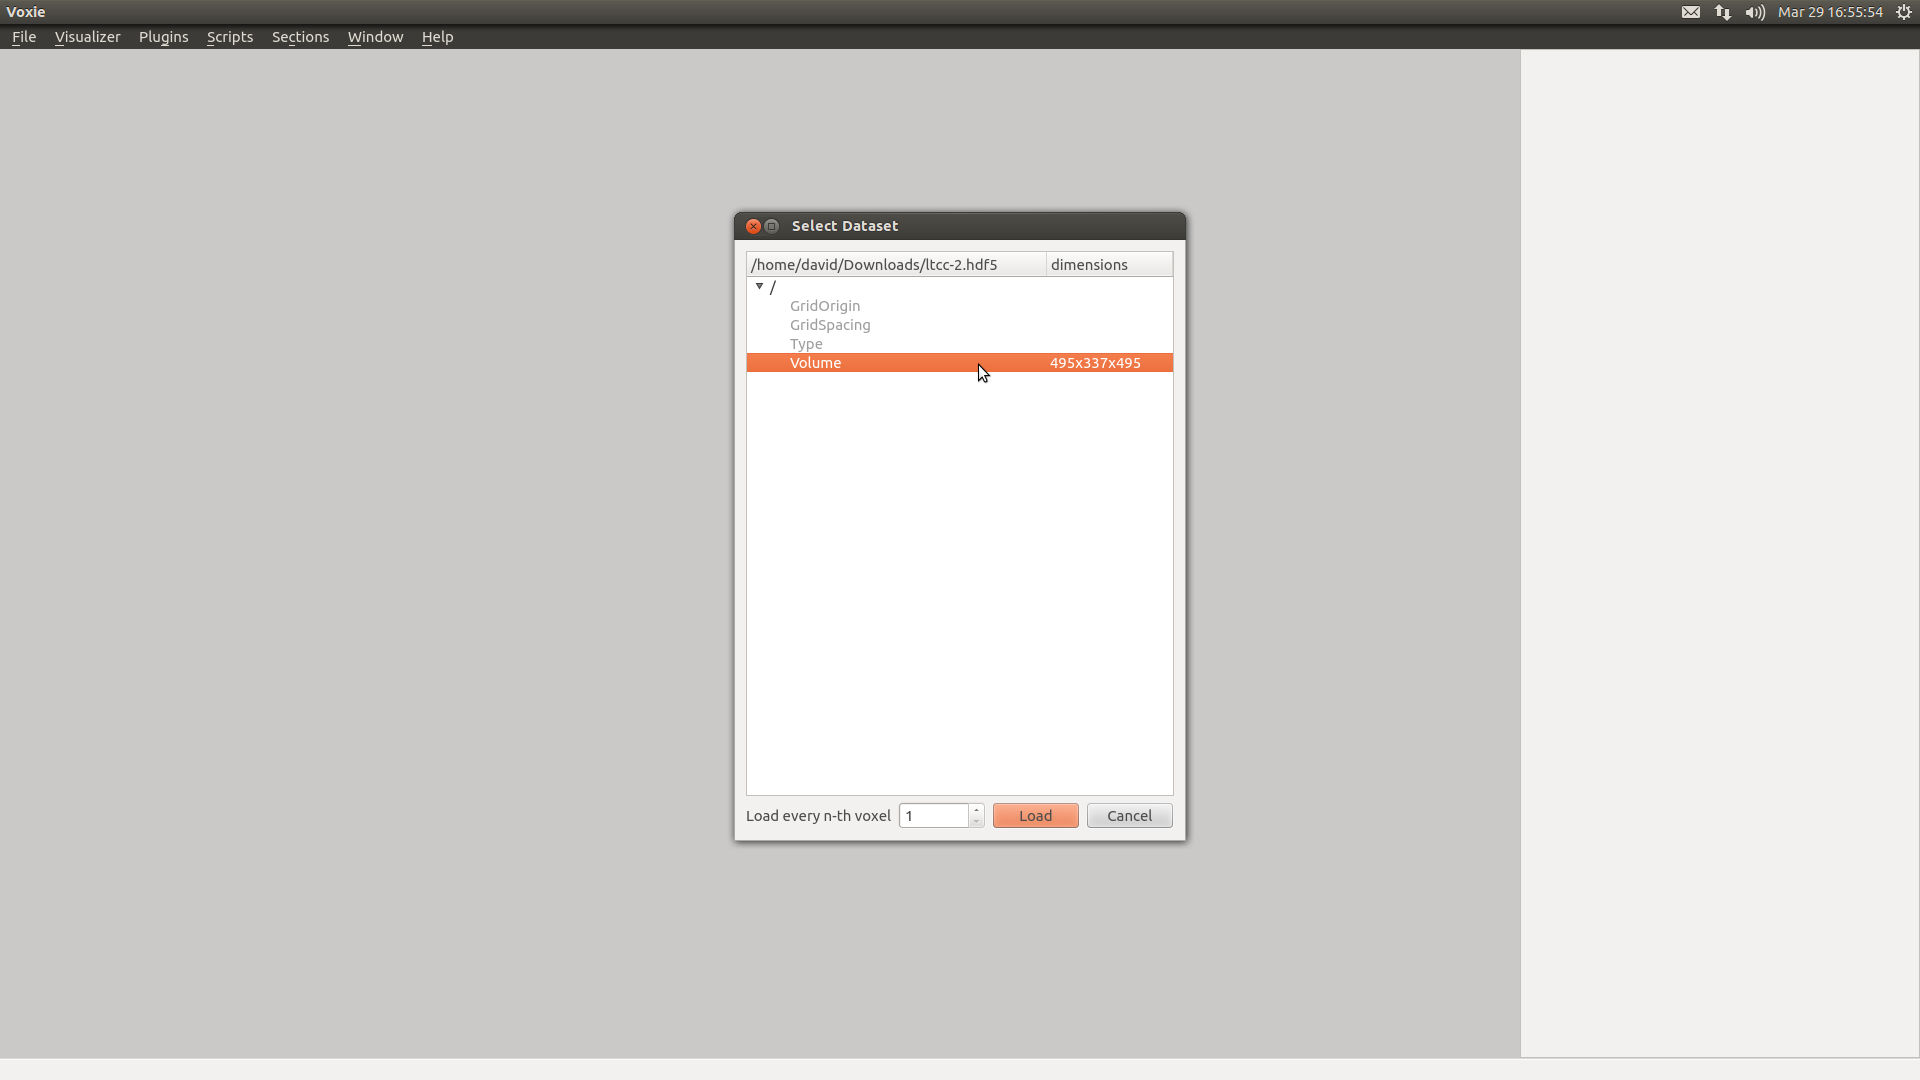
\includegraphics[width=1.0\textwidth]{img/hdf5-dialog.png}
  \caption{HDF5 Dialog}
  \label{hdf5-dialog}
\end{figure}

\begin{figure}[!htbp]
  \centering
  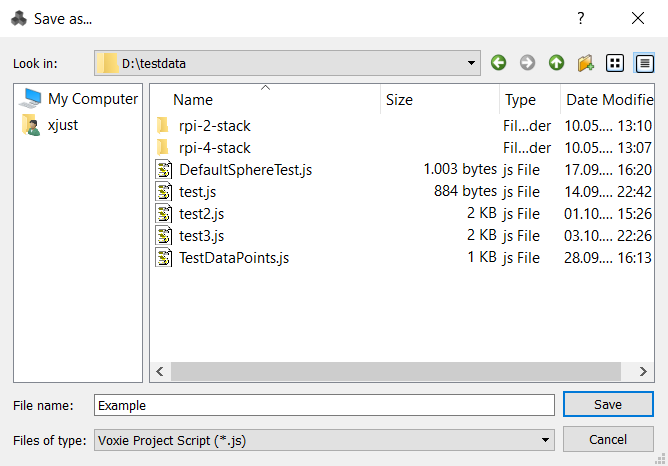
\includegraphics[width=1.0\textwidth]{img/save-dialog.png}
  \caption{Save Voxie Project Dialog}
  \label{save-dialog}
\end{figure}



% Achso und dann noch hdf5 Datei laden

\subsubsection{Visualizer}

The visualizer menu contains sorted entries to create new visualizers.
Visualizers are ordered in 4 categories:
\begin{itemize}
  \item{\emph{2D} \newline Visualize voxel data in 2D.}
  \item{\emph{3D} \newline Visualize voxel data in 3D.}
  \item{\emph{Analytic} \newline Analyze the voxel data without a graphical visualization.}
  \item{\emph{Miscellaneous} \newline Every kind of visualizer that does not fit
    in the above categories }
\end{itemize}

\subsubsection{Plugins}

This menu shows an entry for each plugin that supports UI Commands.
Each entry contains all UI commands for that plugin.

The UI command will be invoked by clicking the command entry.

\subsubsection{Scripts}

This menu allows to show the scripting console which is explained in \ref{scripting-window}.

It also shows all files that reside the folder \emph{scripts} next
to the voxie executable. A click on a script will execute it.

JavaScript (*.js) files are shown by default and will be executed by the
internal JavaScript scripting engine.

Other scripts can be configured to be shown in the menu by setting up a new
script type in the \emph{Scripting}-Section of the preferences window (See \ref{preferences-window}). The files will be executed by starting the external
application defined there.

\subsubsection{Sections}

The \emph{Sections} menu will show all currently active sections.
A click on the menu item will show or hide the section in the side panel.

\subsubsection{Windows}

This menu allows to reorder all currently opened visualizer windows in 4 styles:
\begin{itemize}
  \item{\emph{Cascade}\newline Will cascade the windows from the top left
    corder to the bottom right corner.}
  \item{\emph{Tile}\newline Will till the windows in a regular grid.}
  \item{\emph{Fill}\newline Will maximize the current window.}
  \item{\emph{Tabbed}\newline Will enable or disable tabbed mode. In tabbed mode,
    all windows are maximized and can be switched with a tab control.}
\end{itemize}

\begin{figure}[h]
  \centering
  \def\tabularxcolumn#1{m{#1}}
  \begin{tabularx}{\linewidth}{@{}cXX@{}}
    \begin{tabular}{cc}
      \subfloat[Cascade]{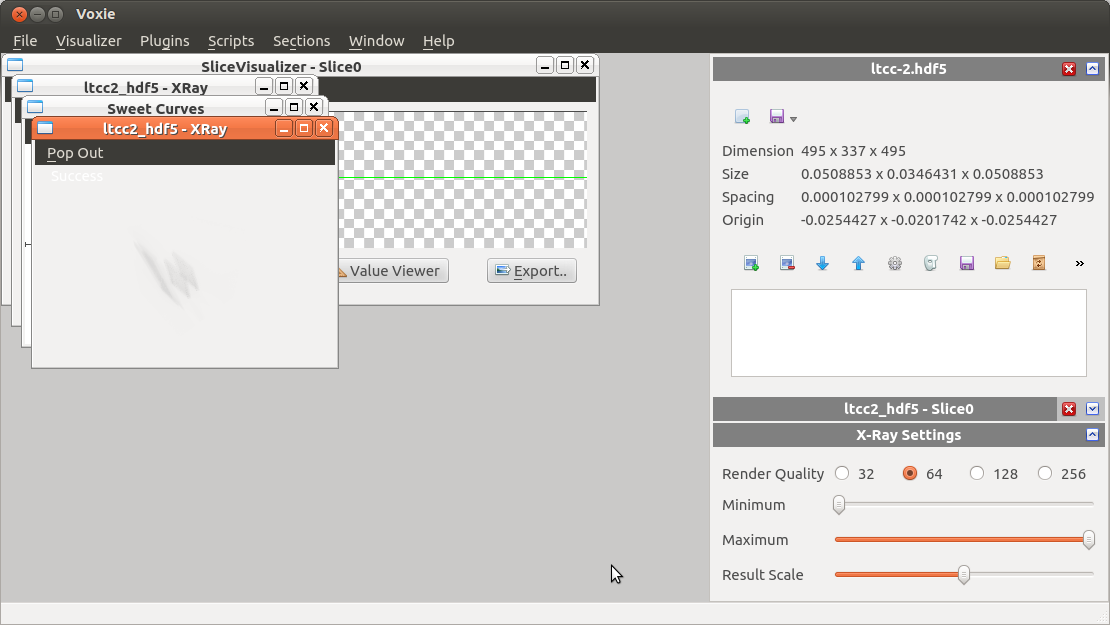
\includegraphics[width=0.5\textwidth]{img/window-cascade.png}} 
      & \subfloat[Tile]{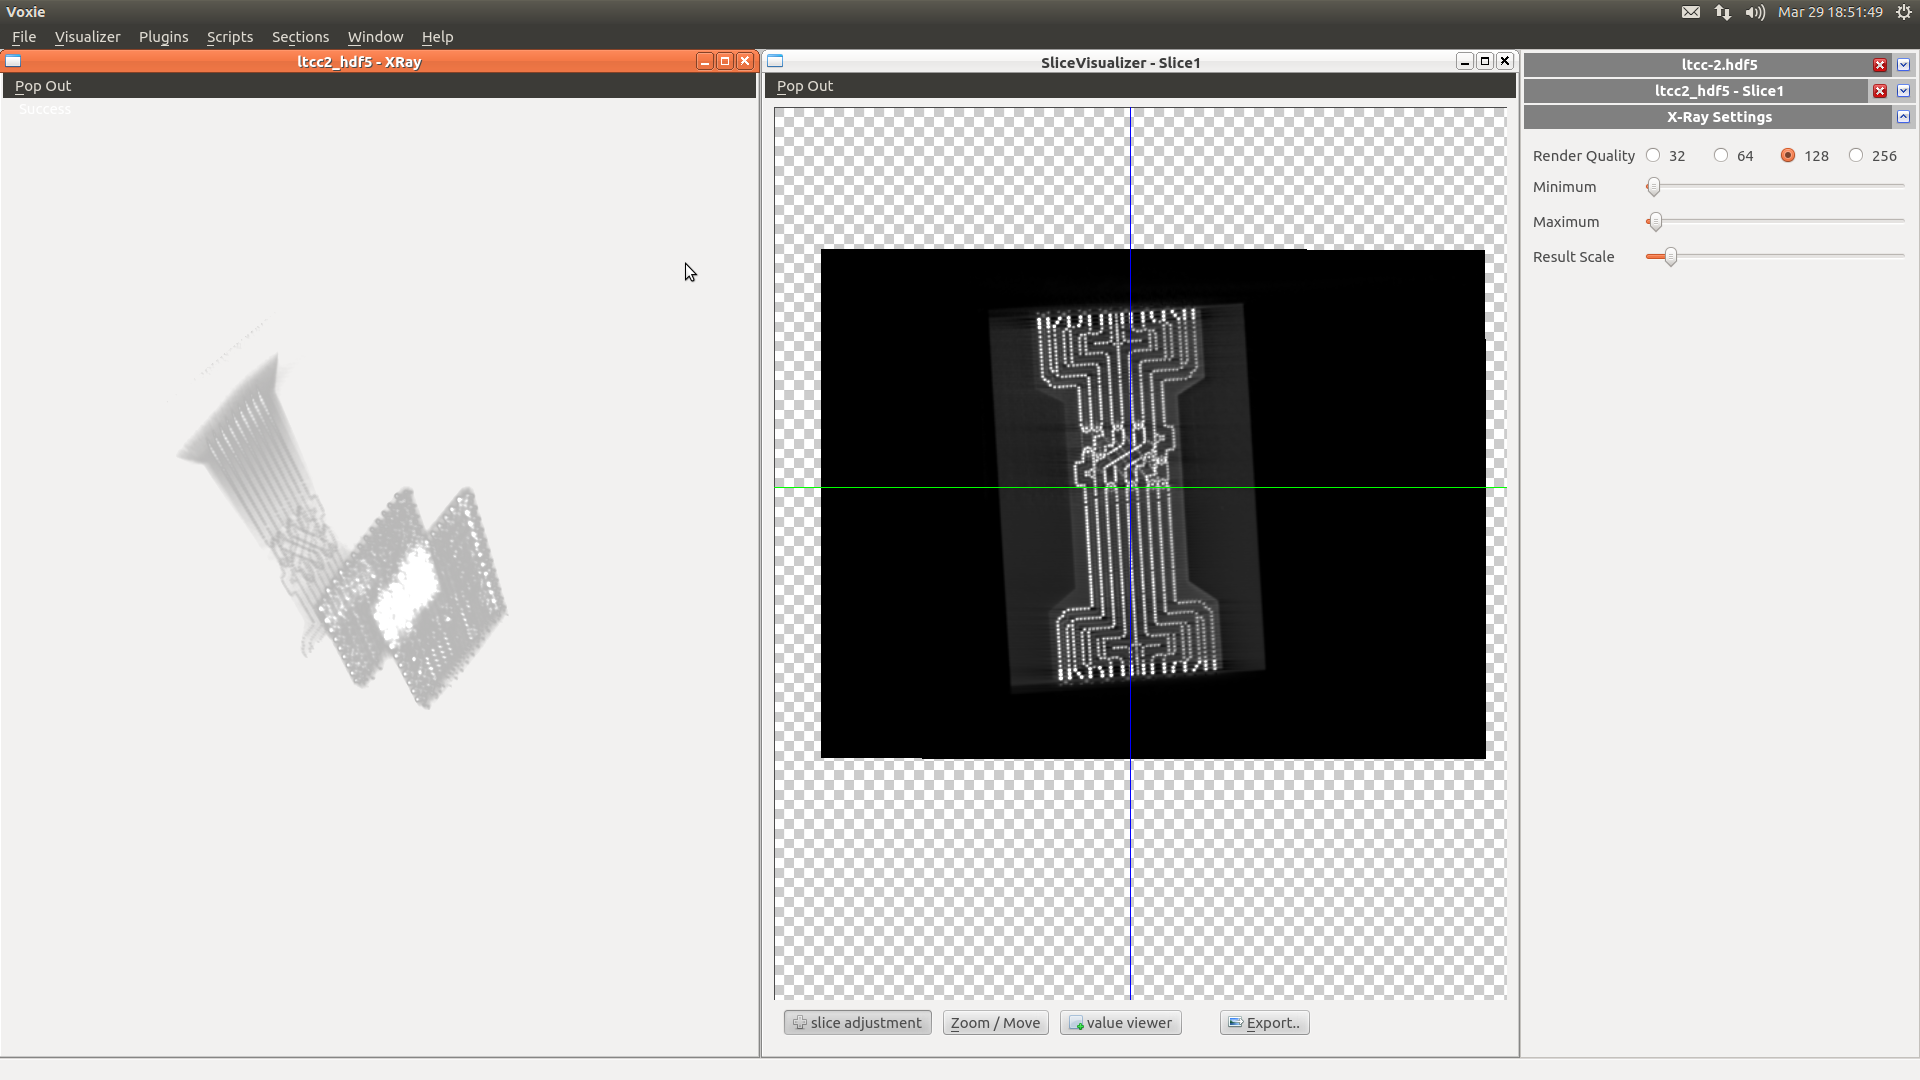
\includegraphics[width=0.5\textwidth]{img/window-tile.png}}\\
      \subfloat[Fill]{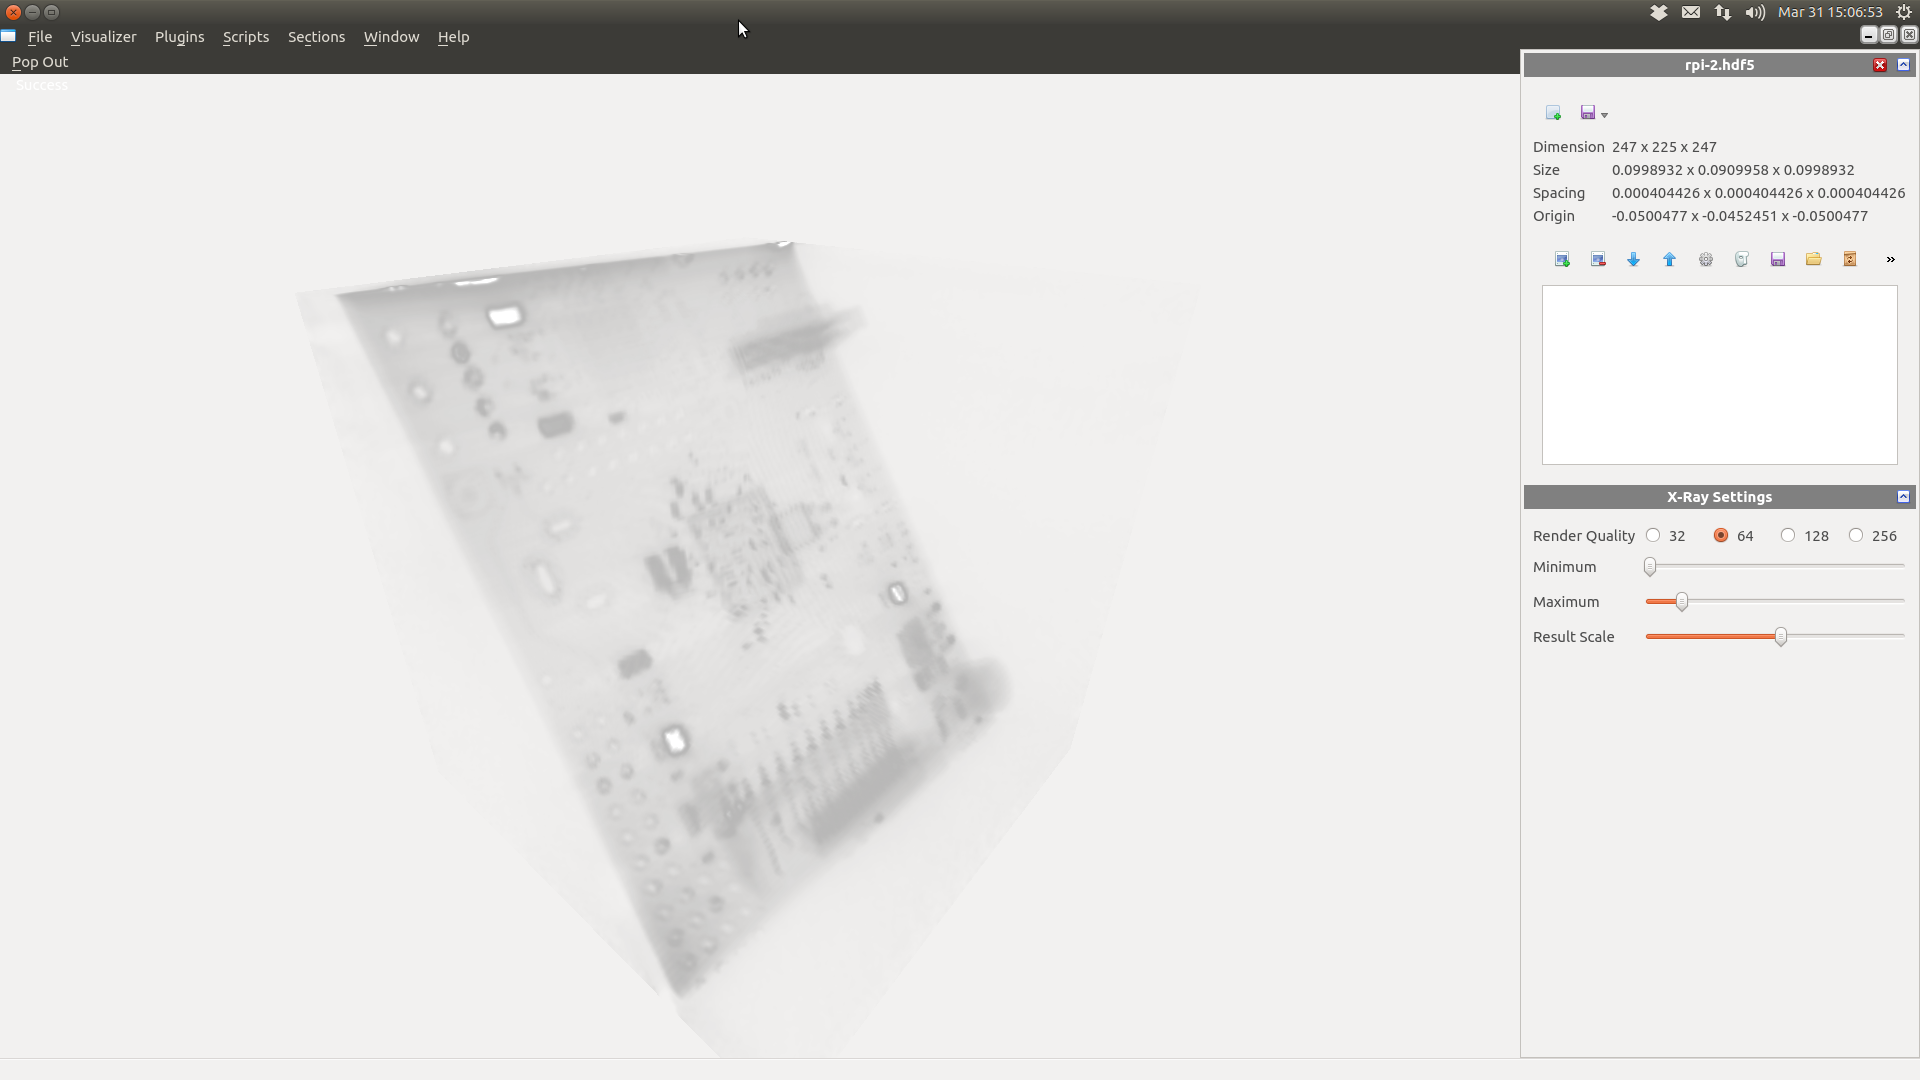
\includegraphics[width=0.5\textwidth]{img/window-fill.png}} 
      & \subfloat[Tabbed]{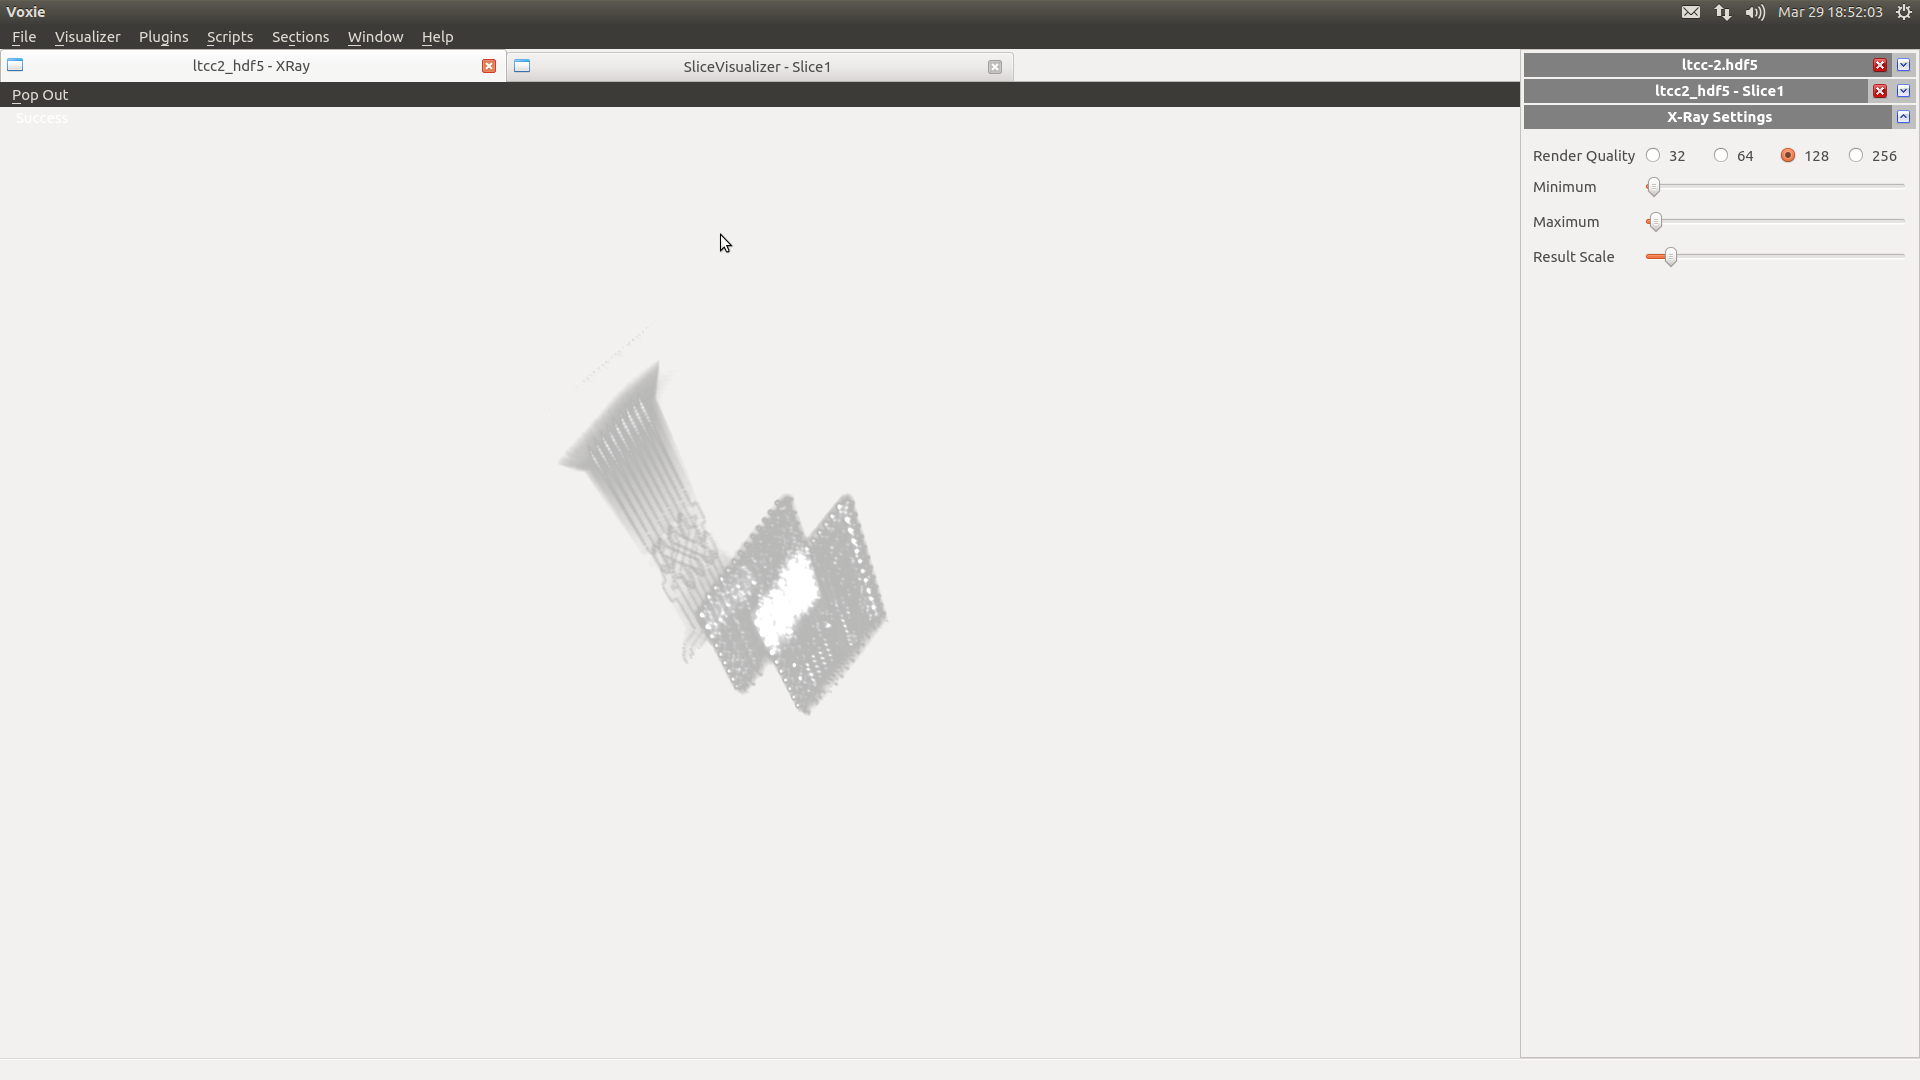
\includegraphics[width=0.5\textwidth]{img/window-tabbed.png}}\\
    \end{tabular}
  \end{tabularx}
  \caption{Window Modes}
  \label{windows-tile}
\end{figure}

\subsubsection{Help}

The help menu offers several possibilites to get help with Voxie:

\begin{itemize}
  \item{\emph{Manuel}\newline Opens this manual.}
  \item{\emph{Wiki}\newline Opens the wiki in the default browser.}
  \item{\emph{About}\newline Shows an about dialog with some quick info about Voxie.}
\end{itemize}

\subsection{Sections}
\label{sections}

Voxie features the side panel, a multifunctional panel showing context dependent
information and settings to the currently active data sets and visualizers.

Sections can be collapsed so they only show their header and may be closable.
If a section gets closed, all data connected will be released (e.g. closing
a data set will close all attached visualizers and slices as well).

% Nur generisch und dataset und slice section

\subsubsection{Data Set Section}

\section{Visualizer}
Voxie comes with 3 standard visualizer plugins included. These plugins feature a 2D Slice visualizer for visualizing single slices, and two 3D visualizers for visualizing 3D datasets, and a 2D raw image visualizer for visualizing raw images.

\subsection{Volume-based visualizer}
Voxie supports the creation of slices. A slice is a plain intersecting the dataset. 
Its visual representation is defined by all voxel values it intersects.

Voxie supports multiple operations on slices. This includes adjusting, filtering, colorizing and analyzing.

\subsubsection{Creating a slice}

A slice is created by telling the data set (VoxelData) to create a new slice. In the UI this is done by clicking on the \textit{Create Slice} button in the section representing the data set.

After adding a slice a new section will appear displaying the position and rotation of the slice. The 3D image describes the position of the slice within the dataset. Values are coded as x (green),  y (blue), z (red). The rotation is displayed as normalized quaternion.

\begin{figure}[h]
	\caption{Slice Section}
	\centering
	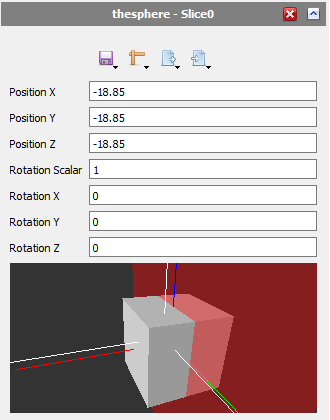
\includegraphics[scale=1.0]{img/2d/3dslice.png}
\end{figure}

\subsubsection{Exporting a slice}

The raw values of the slice can be exported in HDF5 format by clicking on the \textit{Save} button in the slice's section.

\subsubsection{Displaying a slice}

To display a slice Voxie's SliceView plugin has to be used. To add a new Slice View click on Visualizer, then 2D, then Slice.

A dialog will appear. Choosing a slice will create a new window and several new sections.

\begin{figure}[h]
	\caption{The Slice View and its sections and tools}
	\centering
	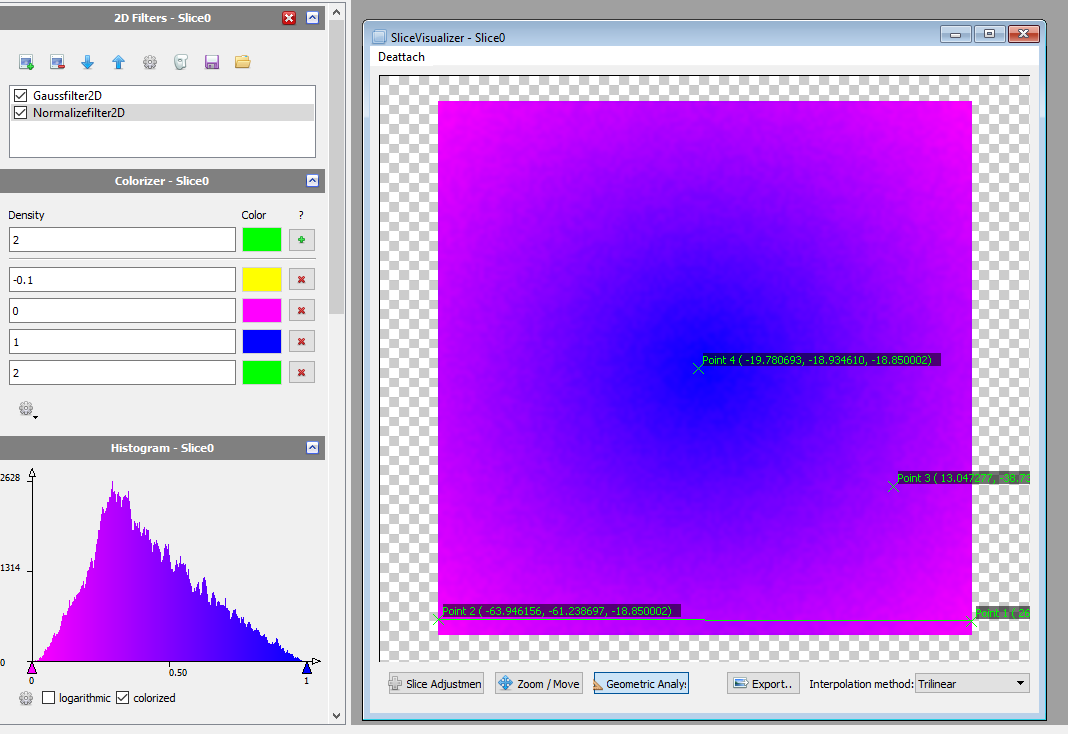
\includegraphics[width=1.0\textwidth]{img/2d/sliceview.png}
\end{figure}


\subsubsection{The slice view}

By default the slice view window offers a canvas that displays the slice associated with the slice view. It also allows for tools to be used which can modify the slice or display information. Tools can be switched by using the number keys.

\subsubsection{Slice Adjustment Tool}
The slice adjustment tool allows for interactive adjustments to be made to the slices configuration.
When this tool is active the x and y axis of the slice are shown (x = green , y = blue). Notice that x points
right and y points down(!).
\\ \\
The slice's origin can be moved to another point on the plane by [right-clicking]. This is useful because the slice's origin is the pivot point for its rotations.\\
The slice's origin can also be moved along its normal vector with the mouse-wheel or [page-up/down] keys. This
Movement can be fine adjusted by holding down [shift] simultaneously.
\\ \\
The slice's rotation can be adjusted an variuos ways.
To rotate the x-y-plane (rotate arround normal vector) hold down [ctrl] and [drag] the mouse with [left-click] arround the origin. \\
This way you can also rotate arround the other axes. To rotate the slice arround the x axis hold down [ctrl]+[x] and drag with [left-click], with [ctrl]+[y]+[left-click][drag] you can rotate arround the y axis. \\
Alternatively you can use the arrow keys [up]/[down]/[left]/[right] to rotate arround the x or y axis. [shift] can be used to slow down the movement with the arrow keys.
\\ \\
For more arbitrary rotation you can "push down" the slice on a specific point with a simple [left-click]. This causes the slice to tilt towards the direction of clicked point (origin is pivot point). To fully understand this imagine the vector that points from the origin to the click point, the vector that is perpendicular to this vector and the normal vector of the plane is the axis of rotation.\\
The step-size can be reduced by holding down [shift]. 

\subsubsection{Zoom / Move Tool}
The zoom and move tool allows one to zoom and move around the displayed image. Holding the left mouse button and dragging will move the image around. The mouse wheel is used to zoom the image. Toggling the checkbox labeled \textit{Drag redraw?} will allow for less processing power to be required as the image will only be altered when the mouse button is released.

\subsubsection{Value Viewer Tool}
The value viewer tool displays values within the image. The value shown below the curser represents the position and the float value of the slice at the given position. Left-clicking will make the value continue to be displayed. Right-clicking will clear all displayed information. Pressing shift shows the unfiltered value. Pressing control will round the position values. Dragging the mouse will calculate the distance between two points in metric distances (see HDF5 specification). Modifying the slice or the generated image will clear all values.

\subsubsection{Mask Selection Tool}
\label{sec:mask}
The Selection Tool allows the User to select an area on the image and on this selected area the filter is applied to. To use this function a filter in the Filter Chain must be selected and only on this filter the mask is applied on. To create a mask you have to click on the mask symbol, then four new buttons appears on the Slice View, \grqq Rectangle\grqq, \grqq Ellipse\grqq, \grqq Polygon\grqq and \grqq Clear\grqq.
\\[12pt]
By clicking on the \textbf{Rectangle Button}, it allows to create a rectangle shape. To do that click and hold the left mouse button and move the mouse. A yellow rectangle appears, this shows the preview of the selection. By realising the left mouse button it finishes the selection and the yellow rectangle turns into red.
\\[12pt]
By clicking on the \textbf{Ellipse Button}, it allows to create a ellipse shape. To do that click and hold the left mouse Button and move the mouse. A yellow ellipse appears, like before it shows the preview of the selection. The first click defines the center of the ellipse. By realising the left mouse button it finishes the selection and the yellow rectangle turns into red.
\\[12pt]
By clicking on the \textbf{Polygon Button}, it allows to create a polygon shape. To do that click on the image, every click is one vertex of the polygon. Every click connects the vertices in yellow, this is just the preview. By pressing space, the polygon shape closes automatically. Notice that at least three vertices are needed to close a polygon shape.
\\[12pt]
By clicking on the \textbf{Clear Button}, it deletes every created shape on the mask only for the selected filter.

\subsubsection{Export Tool}

The export tool will allow for the currently displayed image to be saved. There are three modes available; filtered image, filtered and colorized image or the whole canvas (including borders outside the image).

\subsubsection{Slice View Sections}

A slice view creates three new sections on initialization.

\begin{itemize}
	\item{\emph{2D Filter }\newline This section allows for definition of filters, their order and masks. An ordered set of filters is called a filterchain.}
	\item{\emph{Colorizer}\newline The colorizer section maps values to colors. In between values will be interpolated.}	
	\item{\emph{Histogram}\newline The value distribution is visualized here. It also offers advanced options like logarithmic scaling.}

\end{itemize}

\begin{figure}[h]
	\caption{2D Filter Section}
	\centering
	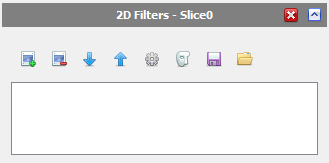
\includegraphics[scale=1.0]{img/2d/2dfilter.png}
\end{figure}

\subsubsection{Adding 2D Filters}

A 2D filter can be added by clicking on the \emph{Add Filter} button will open a dialogue allowing one to choose what kind of filter is to be added. Filters are automatically active after creation.

\subsubsection{Removing 2D Filters}

Filters can be removed by highlighting a filter in the section then clicking the \emph{Remove Filter} button.

\subsubsection{Choosing which Filters to apply}

Filters can be temporarily deactivated by toggling the checkbox next to their name.

\subsubsection{Ordering 2D Filters}

Filters are applied in order from top to bottom. Their ordering can be altered by highlighting a filter then pressing the array buttons to move them up or down.

\subsubsection{Configuration of 2D Filters}

Some filters posses a configuration dialogue. The dialogue can be opened by highlighting the desired filter then pressing the \emph{Options} button (\emph{Wheel}).

\subsubsection{Loading and saving Filterchains}

Filterchains including the individual filter settings can be exported and imported using the \emph{Export Filterchain} and \emph{Import Filterchain} buttons. The filterchain will be represented by a human readable xml file.

\subsubsection{Filter Masks}

After activating the filter feature by adding filters, the \emph{Filter Mask} button will activate the filter mask feature in the slice view. This allows for the \emph{Mask Selection Tool} to be used. See \ref{sec:mask} for more information.

\begin{figure}[h!]
	\caption{Colorizer Section}
	\centering
	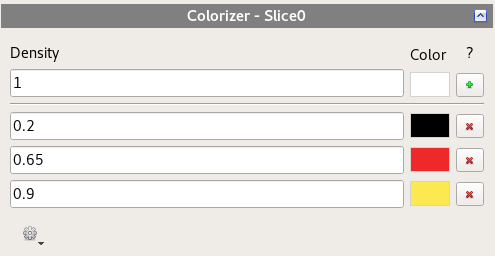
\includegraphics[scale=1.0]{img/2d/colorizer.png}
\end{figure}

\subsubsection{Colorizer}

The colorizer maps values to colors. Colors in between the given mappings will be interpolated. Mapping can be added by pressing the \emph{Add Mapping} button in the first column. This will add a new mapping to the list of mappings below.\newline The colors can be changed by clicking on the displayed color. This will invoke the operating system specific color picker. \newline To remove a mapping simply click on the \emph{Remove Mapping} button. \newline Please note that mappings with the same value will be automatically merged, the new mapping having priority.

\subsubsection{Histogram}

The histogram section shows a visualization of the value distribution of the slice. The scale can be set to be linear or logarithmic. Upper and lower bound as well as the maximum count value can be set via dialogue.
 
\subsubsection{Displaying the difference between two slices}

If two Slices should be compared, the DiffView plugin has to be used. To add a new DIff View click on Visualizer, then 2D, then DiffView.

A dialog will appear. Choosing two slices will create a new window and several new sections.

The DiffView is build similar to the SliceView, thereforce the following subsctions only describe the changes between the DiffView and the SliceView.


\subsubsection{Slice Adjustment Tool}

The Slice Adjustment Tool within the DiffView brings two new buttons: "Switch Slice" to switch the slice that is currently adjusted and "Select Both" to adjust both slices at the same time.

The Origin of the currently not altered Slice will be shown as DashLine. 

\subsubsection{Value Viewer Tool}
The value viewer for the DiffView will always display two values, as there are two Slices, except if the Shift-Key is pressed, then the value for the filtered Image (which is not connected to a slice anymore) will be shown.

\subsection{Raw-based visualizer}
Voxie supports the display of raw images. A raw image is a single projection from the ct.
Its visual representation is defined by its pixel values.

Voxie supports multiple operations on raw images. This includes adjusting, colorizing, analyzing.

\subsubsection{Creating a raw visualizer}

A raw visualizer is created by opening a file which contains raw images. In the UI this is done by right clicking in the object tree and pressing on \textit{Open File} and select the file.
After loading the file, click right on it in the object tree and press create \textit{Create Rawvisualizer}. 

\subsubsection{The raw image view}

By default the raw image view window offers a canvas that displays the raw associated with the raw image view. It also allows for tools to be used which can modify the slice or display information. Tools can be switched by using the number keys.

\subsubsection{Zoom / Move Tool}

The zoom and move tool allows one to zoom and move around the displayed image. Holding the left mouse button and dragging will move the image around. The mouse wheel is used to zoom the image. Toggling the checkbox labeled \textit{Drag redraw?} will allow for less processing power to be required as the image will only be altered when the mouse button is released.

\subsubsection{Slice View Sections}

A slice view creates six new sections on initialization.

\begin{itemize}
  \item{\emph{Select Picture\newline The select picture section allows to select a new picture by its number and shows it after it has been loaded.}}
  \item{\emph{Colorizer}\newline The colorizer section maps values to colors. In between values will be interpolated.}
  \item{\emph{Histogram}\newline The value distribution is visualized here. It also offers advanced options like logarithmic scaling.}
  \item{\emph{Options menu}\newline The menu includes two sliders which can adjust the rate of the slide show speed and the amount of buffered raw images. There is also a button to stop all queue loading operations for this dataset. For the change of the buffer size to go in effect the apply button needs to be pressed. Warning: Changing the buffers size may affect your performance depending on your computer specifications.}
\end{itemize}

\subsubsection{Colorizer}

The colorizer maps values to colors. Colors in between the given mappings will be interpolated. A color mapping can be added by pressing the \emph{Add Mapping} button in the first column. This will add a new mapping to the list of mappings below.\newline The colors can be changed by clicking on the displayed color. This will invoke the operating system specific color picker. \newline To remove a mapping simply click on the \emph{Remove Mapping} button. \newline Please note that mappings with the same value will be automatically merged, the new mapping having priority. \newline A click on the gear button opens a small options menu with two options: \emph{Calculate Mapping} automatically calculates a color mapping of two values by using an algorithm based on the whole 3D dataset. \emph{Default mapping} removes the color mapping and replaces it with the default one (0 = black, 1 = white).

\begin{figure}[h!]
  \centering
  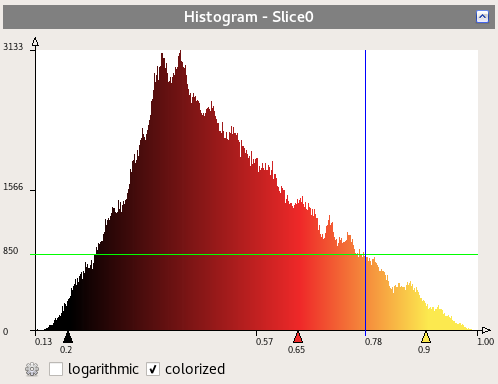
\includegraphics[scale=0.5]{img/2d/histogram}
  \caption{Histogram Section}
\end{figure}  

\subsubsection{Histogram}

The histogram section shows a visualization of the value distribution of the slice. The scale can be set to linear or logarithmic by switching the \emph{logarithmic} check box. 
\newline The histogram can be colorized dependant on the color mapping values by activating the \emph{colorized} check box. The color mapping (adjusted in the Colorizer) is also permanently shown along the X-Axis as colored triangles.\newline Points within the histogram widget can be marked by a left click with the mouse in the desired area. Move the marker by holding the left mouse button. The related values are shown down the x and y axis. Deleting a marked point works by right clicking with the mouse inside the histogram widget.\newline A gear symbol opens the options dialog. By default, the bouds of the axes are calculated automatically in a way that all values are displayed within the histogram widget. Manual bounds are possible by deactivating the \emph{automatic} checkboxes and setting specific values in the related text boxes. \newline The non-colorized histogram is red by default without a background color. Those color values are adjustable manually by clicking on the colored boxes. \newline The histogram widget can be adjusted in height. This is useful for accurate work.\newline \emph{Hint: All values are applied in real time. Watch the histogram while adjusting the values to get better results}.

\begin{figure}[h!]
  \centering
  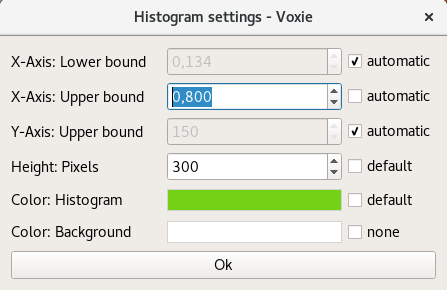
\includegraphics[scale=0.5]{img/2d/histosettings}
  \caption{Histogram Options}
\end{figure}  

\subsubsection{Change image toolbar}

The toolbar is attached below the raw image view and consists of three buttons

\begin{itemize}
\item Forwards button
\item Backwards button
\item Start/Stop slide show button 
\end{itemize}

The forwards/backwards button both move through the pictures in the respective direction. The visualizer also stores how many times you pressed a button, meaning if you press 10x the forward button the visualizer will show as soon as the pictures are available, the next 10 picture originating from your current picture.
The start/stop button starts or stops the slide show which loops through the entire raw dataset. If too many loading commands were executed, it is possible to clear them all out by pressing the \textit{Clear Queue} button in the options menu in the sidebar.

\subsection{3D}
% TODO BY FELIX

3D visualizers allow the user to get a an idea of the data set they are working with.
The visualizers don't allow exact measurement or inspection but they provide enough
information to get how the data set look.

\subsection{Isosurface}

The isosurface visualizer allows display of an isosurface. Isosurfaces are
surfaces in data sets with equal density. This allows displaying structures of
similar or equal density as a solid object.

\subsubsection{Settings}
The Isosurface visualizer can be set up via its side panel section.
The section has multiple options:
\begin{itemize}
	\item{\emph{Threshold}\newline The threshold value for the isosurface.}
	\item{\emph{Method}\newline The method used for generating the isosurface.}
	\item{\emph{Invert}\newline A flag that determines if the surface is built
		against values below the threshold or above the threshold.}
	\item{\emph{Refresh}\newline Refreshes the isosurface model.}
\end{itemize}
The Isosurface visualizer needs some time to generate an isosurface so it does not
view anything by default.
The visualizer needs to be set up and then the \emph{Refresh}-Button must be pressed
to regenerate the isosurface model.

\subsubsection{Controls}
The data set can be rotated by dragging the mouse over the visualizer window while
holding down the left mouse button.
Scrolling the mouse wheel will zoom in or out the view.

\begin{figure}[h!]
	\caption{Isosurface}
	\centering
	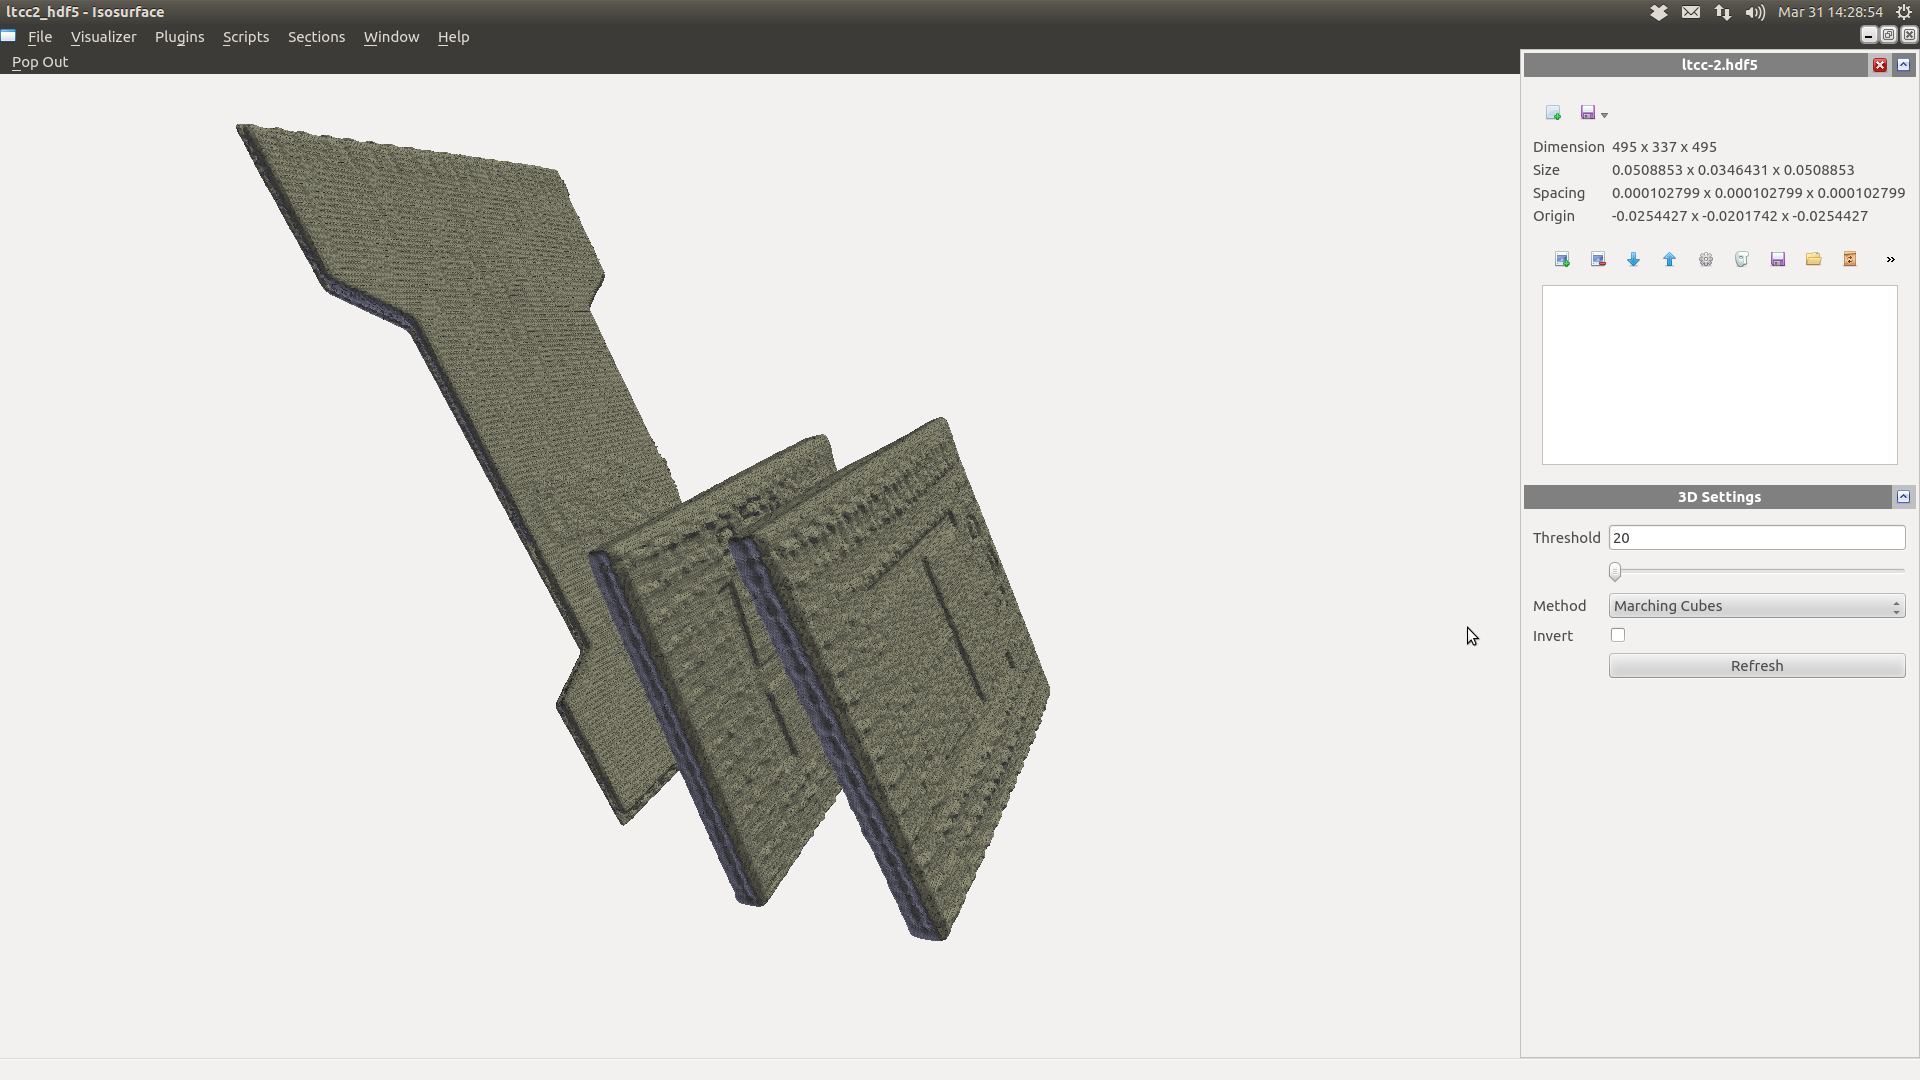
\includegraphics[width=1.0\textwidth]{img/isosurface.png}
\end{figure}

\newpage
\subsection{X-Ray}

The X-Ray visualizer allows seeing the data set as a whole piece. It accumulates
the voxels it finds while raycasting into the scene and thus shows the interior of
the data set.

It is useful to gather information about where specific structures are located in
the data set, if there are cavities in the data set or points with a high density.

\subsubsection{Settings}
The X-Ray visualizer can be set up via its side panel section.
The section has multiple options:
\begin{itemize}
	\item{\emph{Render Quality}\newline The number of samples used by the raycaster.
		Lower values are faster, higher values give more details.}
	\item{\emph{Minimum}\newline The minimum value considered as black/transparent.
		Can be used as an additional high-pass filter.}	
	\item{\emph{Maximum}\newline The maximum value considered as white/opaque.
			Can be used as a range adjustment.}
	\item{\emph{Result Scale}\newline Scales the result from the range options by
		a given amount. Can be used to tweak the image brightness.}
\end{itemize}
The settings the of visualizer are unit-less as the visualizer only provides a
visual representation that must be tweaked by eye.

For a computationally under-performing computer it is recommended to not use the
higher render quality settings as they draw a lot of computational power.

\subsubsection{Controls}
The data set can be rotated by dragging the mouse over the visualizer window while
holding down the left mouse button.
Scrolling the mouse wheel will zoom in or out the view.

\begin{figure}[h!]
	\caption{X-Ray}
	\centering
	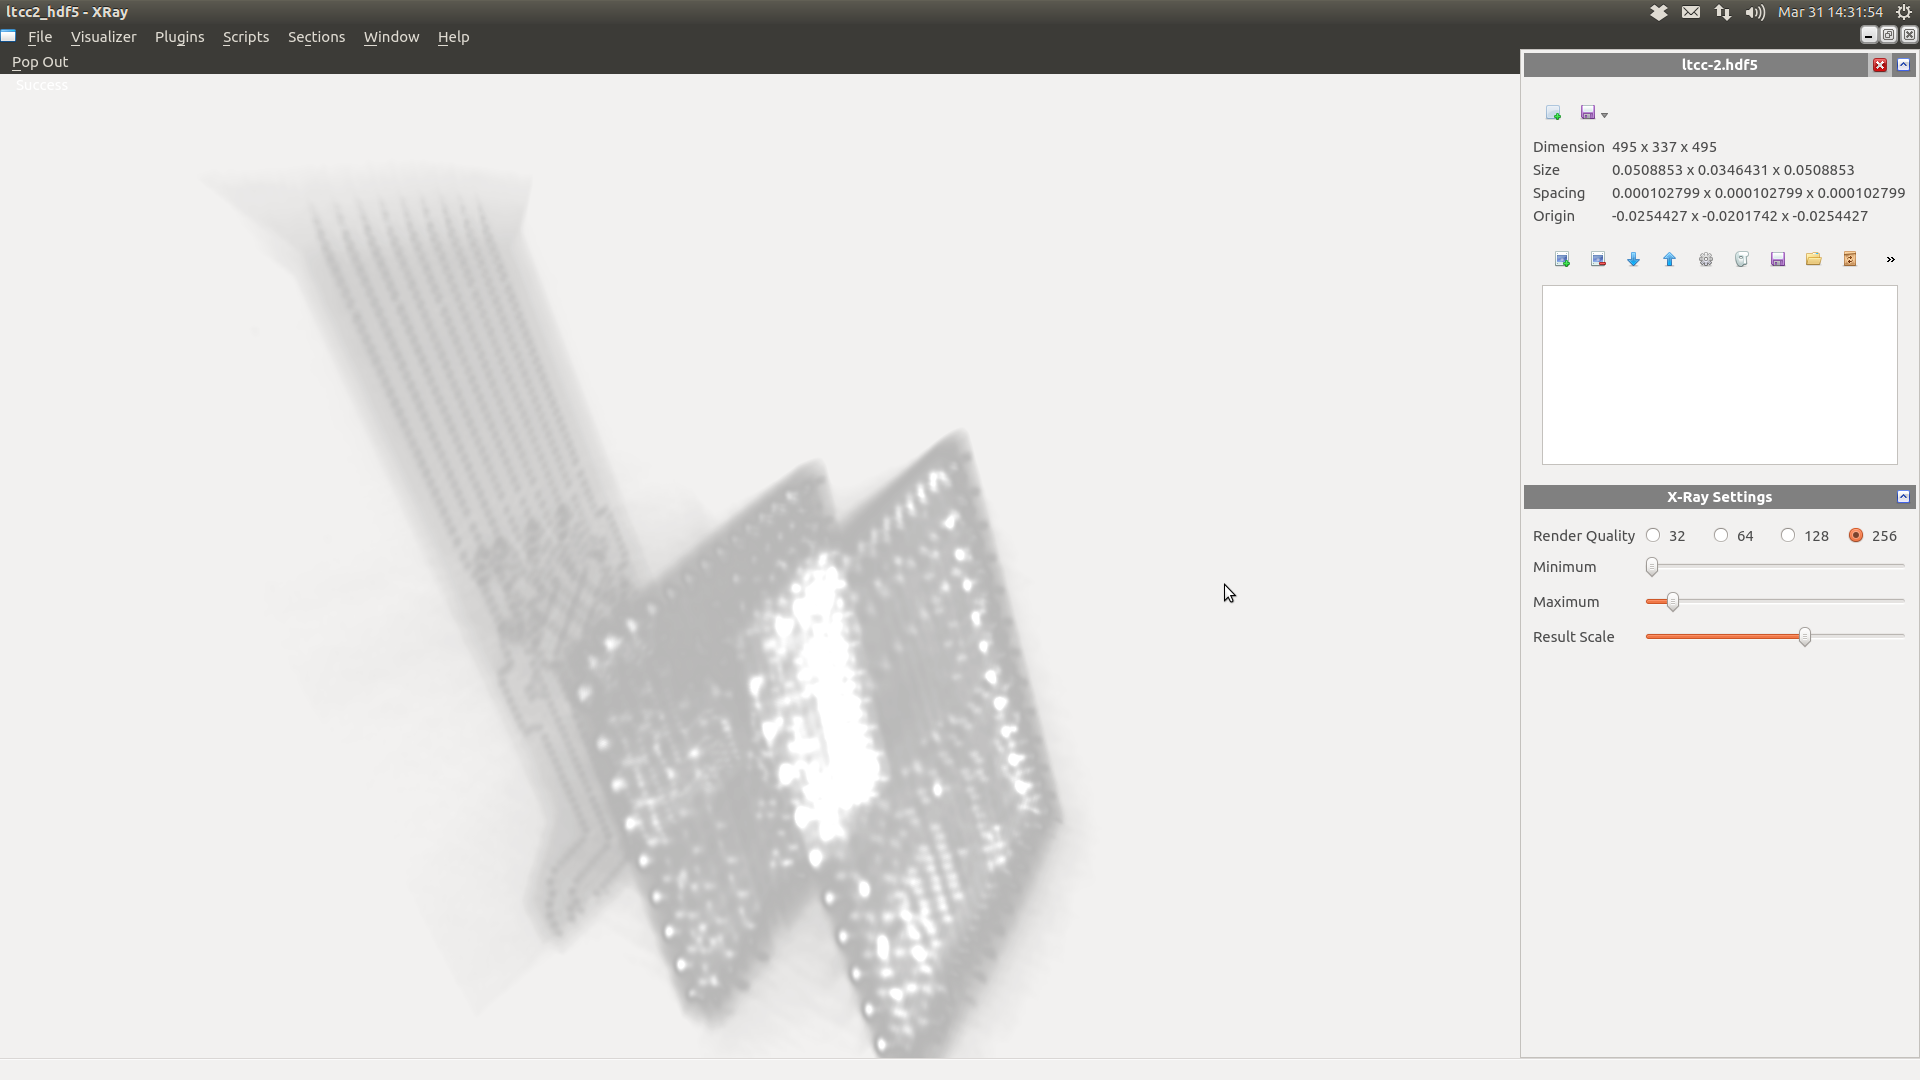
\includegraphics[width=1.0\textwidth]{img/x-ray.png}
\end{figure}
\section{Appendix}
\subsection{Definitions}
\subsubsection*{Cutting Planes}\label{sec:def_cuttingplane}
A cutting plane is a plane which cuts the surface of a data set in two parts and hides one of these parts. (see \autoref{fig:cuttingplane_cube})

\begin{figure}[h!]
  \centering
  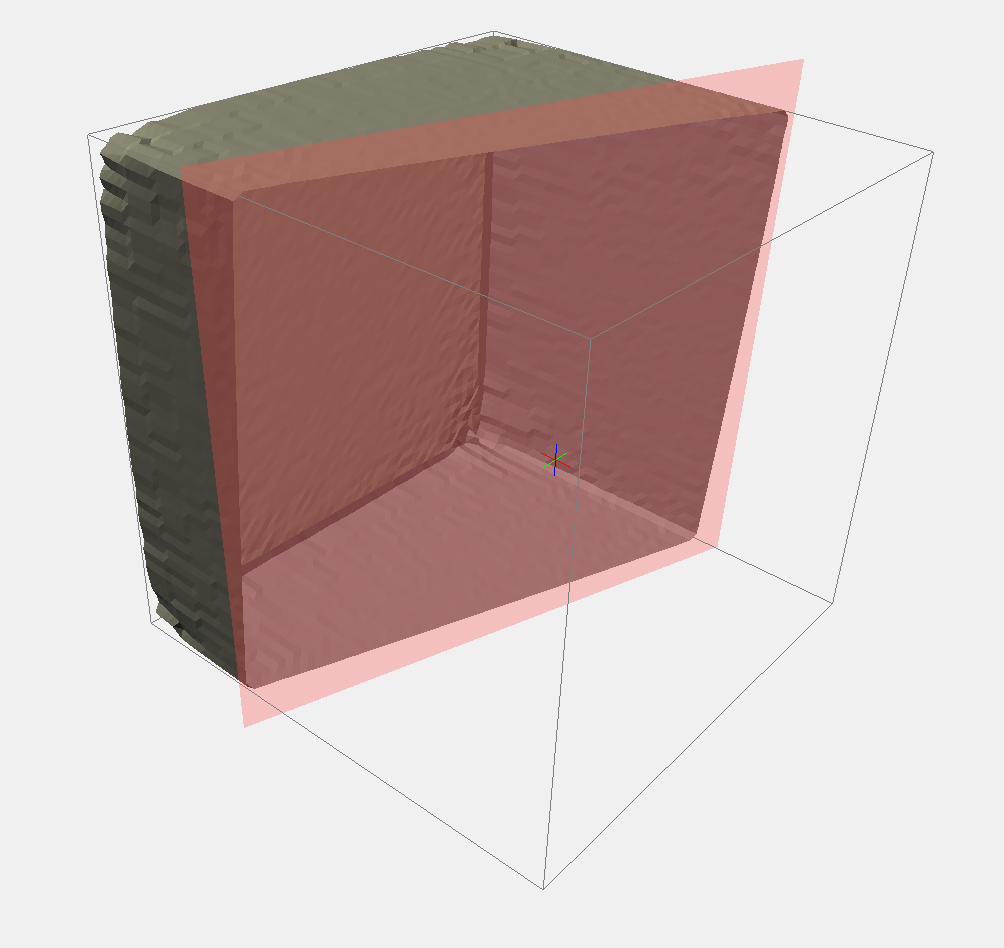
\includegraphics[width=1.0\textwidth]{img/cuttingplane_cube.png}
  \caption{A cutting plane cutting away the front part of a cube}
  \label{fig:cuttingplane_cube}
\end{figure}

%\section{Scripting}
%\input{scripting.tex}
%\section{Plugins}
%Here be plugins

\label{ui-command}

\end{document}
